%! alt The lower-bound construction drawn small: three red points, labelled R and drawn in the accent colour, and three blue points, labelled B, alternate around a circle, and one more blue point lies off the circle. Every chord joining neighbouring points on the circle joins two colours, so some line must cross it. The highlighted line crosses exactly two sides of the hexagon formed by the six points, and no line can cross more than two.
%! after_paragraph 2
%! scale 1
% The shared preamble of every Cevian figure. pipeline/figures turns these colours into theme-aware paint,
% and refuses any other colour, so draw only with them:
%   figink (lines and labels), figaux (construction lines), figaccent (the object the argument turns on),
%   figtint and figaccenttint (light fills).
\documentclass[border=1.5pt]{standalone}
\usepackage{tkz-euclide}
\definecolor{figink}{RGB}{0,0,0}
\definecolor{figaux}{RGB}{85,85,85}
\definecolor{figaccent}{RGB}{192,57,43}
\definecolor{figtint}{RGB}{221,221,221}
\definecolor{figaccenttint}{RGB}{245,213,208}
% tkz-euclide's defaults draw circles, compasses and marks in 50% grey and fill points with a tint.
\makeatletter
\def\tkz@otherlinecolor{figink}
\def\tkz@euc@circlecolor{figink}
\def\tkz@euc@compasscolor{figink}
\def\tkz@euc@mkcolor{figink}
\def\tkz@mk@fill{figink}
\def\tkz@euc@pointfillcolor{figink}
\makeatother
\tkzSetUpLine[color=figink,line width=.7pt]
\tkzSetUpArc[color=figink,line width=.7pt]
\tkzSetUpCompass[color=figink,line width=.5pt]
\tkzSetUpPoint[color=figink,fill=figink,size=3.1pt]
\tikzset{
  every picture/.style={line cap=round,line join=round,color=figink},
  circle style/.append style={color=figink,line width=.7pt},
  aux/.style={color=figaux,line width=.45pt,dash pattern=on 2.6pt off 2pt},
  key/.style={color=figaccent,line width=1pt},
  mk/.style={color=figink,line width=.5pt},
  lbl/.style={color=figink,inner sep=2.2pt},
  len/.style={color=figink,inner sep=1.5pt,font=\small},
}

\begin{document}
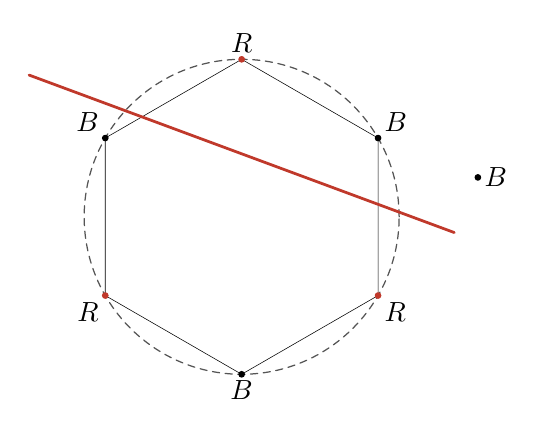
\begin{tikzpicture}
\tkzDefPoint(0.0,0.0){O} %! O = (0, 0)
\tkzDefPoint(0.0000000000000000000000000000000000000000000000000043348337,2.0000000){P1} %! P1 = polar(O, 2, 90)
\tkzDefPoint(-1.7320508,1.0000000){P2} %! P2 = polar(O, 2, 150)
\tkzDefPoint(-1.7320508,-1.0000000){P3} %! P3 = polar(O, 2, 210)
\tkzDefPoint(-0.000000000000000000000000000000000000000000000000013004501,-2.0000000){P4} %! P4 = polar(O, 2, 270)
\tkzDefPoint(1.7320508,-1.0000000){P5} %! P5 = polar(O, 2, 330)
\tkzDefPoint(1.7320508,1.0000000){P6} %! P6 = polar(O, 2, 30)
\tkzDefPoint(3.0000000,0.50000000){X} %! X = (3, 1/2)
\tkzDefPoint(-2.7000000,1.8000000){L1} %! L1 = (-27/10, 9/5)
\tkzDefPoint(2.7000000,-0.20000000){L2} %! L2 = (27/10, -1/5)
%! fact on_circle(P1, O, 2)
%! fact on_circle(P4, O, 2)
\tkzDrawCircle[aux](O,P1)
\tkzDrawPolygon(P1,P2,P3,P4,P5,P6)
\tkzDrawSegment[key](L1,L2)
\tkzDrawPoints(P2,P4,P6,X)
\tkzDrawPoints[color=figaccent,fill=figaccent](P1,P3,P5)
\tkzLabelPoint[above,lbl](P1){$R$}
\tkzLabelPoint[above left,lbl](P2){$B$}
\tkzLabelPoint[below left,lbl](P3){$R$}
\tkzLabelPoint[below,lbl](P4){$B$}
\tkzLabelPoint[below right,lbl](P5){$R$}
\tkzLabelPoint[above right,lbl](P6){$B$}
\tkzLabelPoint[right,lbl](X){$B$}
\end{tikzpicture}
\end{document}
